\newcommand{\nrandom}{\num{700}}
\newcommand{\napplication}{\num{120}}
\newcommand{\nstrategic}{\num{60}}
\newcommand{\npec}{\num{60}}

\begin{frame}
    \frametitle{Evaluation}
    \begin{itemize}
        \item Compared solvers
              \begin{itemize}
                  \item \ressat: \texttt{C++} language inside~\abc environment~\cite{ABC}
                        \begin{itemize}
                            \item SAT solver: \minisat-2.2~\cite{Een2003Solver}
                            \item Weighted model counter: \cachet~\cite{Sang2004}
                        \end{itemize}
                  \item \ressatb: \ressat without minterm generalization
                  \item \dcssat: state-of-the-art DPLL-based SSAT solver
              \end{itemize}
              \pause
        \item Experimental setup
              \begin{itemize}
                  \item A machine with~\machineSpec
                  \item \osInfo
                  \item CPU time: \timelimit; memory: \memlimit
              \end{itemize}
    \end{itemize}
\end{frame}

\begin{frame}
    \frametitle{Benchmark Set}
    \begin{itemize}
        \item Random $k$-CNF formulas (by \cnfgen~\cite{Lauria2017CNFgen})
              \begin{itemize}
                  \item $k\in\{3,\ldots,9\},n\in\{10,20,\ldots,50\},\frac{m}{n}=\{k-1,k,k+1,k+2\}$
                  \item Quantify half variables randomly and others existentially
                  \item \num{5} samples per configuration: \nrandom~formulas
              \end{itemize}
              \pause
        \item Strategic-company~\cite{Cadoli1997} formulas
              \begin{itemize}
                  \item Forall-exist QBF: decide whether a company is \textit{strategic}
                  \item Replace universal quantifiers with randomized ones
                  \item From \texttt{QBFLIB}~\cite{Narizzano2006}: \nstrategic~formulas
              \end{itemize}
              \pause
        \item PEC formulas: \npec~formulas
    \end{itemize}
\end{frame}

\begin{frame}
    \frametitle{Implications from the Results}
    \begin{itemize}
        \item \ressat outperforms \dcssat on random and strategic formulas
              \pause
        \item \ressat is able to derive non-trivial bounds when \dcssat timeouts
              \pause
        \item Minterm generalization is crucial to the performance of \ressat
    \end{itemize}
\end{frame}

\begin{frame}
    \frametitle{Quantile Plot for Random Formulas}
    \begin{figure}
        \centering
        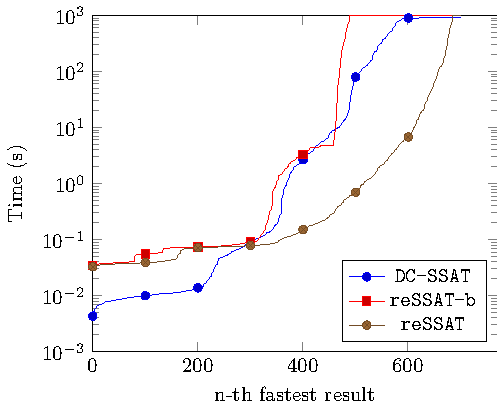
\includegraphics{fig/random-exist-ssat/quantile-cputime-Random.pdf}
    \end{figure}
\end{frame}

\begin{frame}
    \frametitle{Quantile Plot for Strategic-Company Formulas}
    \begin{figure}
        \centering
        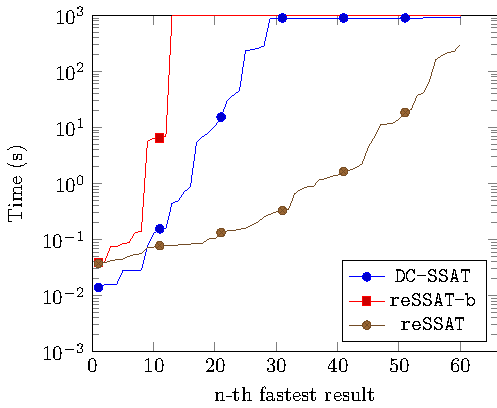
\includegraphics{fig/random-exist-ssat/quantile-cputime-Strategic.pdf}
    \end{figure}
\end{frame}

\begin{frame}
    \frametitle{Results for PEC Formulas ($\dr=0.01$)}
    \begin{table}[ht]
        \centering
        \tiny
        \pgfplotstabletypeset[
            every head row/.style={before row={\toprule
                            & \multicolumn{4}{c}{\dcssat} & \multicolumn{6}{c}{\ressat} & \multicolumn{6}{c}{\ressatb}\\},after row=\midrule},
            every last row/.style={after row=\bottomrule},
            every row no 0/.style={before row={\rowcolor{yellow}}},
            every row no 10/.style={before row={\rowcolor{yellow}}},
            empty cells with={--},
            formula column/.list={0},
            time column/.list={1,3,6},
            prob column/.list={2,4,7},
            ubound column/.list={5,8}
        ]
        {random-exist-ssat/parsed-PEC-0.01.csv}
    \end{table}
\end{frame}